\documentclass[10pt, aspectratio=169]{beamer}
\usetheme[
  sectionpage=progressbar,
  numbering=fraction,
  progressbar=none,
  block=fill,
]{metropolis} % Use metropolis theme

% ------------------------------------------------------------------------------
% Packages
% ------------------------------------------------------------------------------
\usepackage[ddmmyyyy]{datetime}
\usepackage[T1]{fontenc}
\usepackage[utf8]{inputenc}

% Page setting
\usepackage[explicit]{titlesec}
\usepackage{sectsty}
\usepackage{fancyhdr}
\usepackage[title, titletoc]{appendix}

% Fonts
\usepackage{kpfonts}
\usepackage{amsmath}
\usepackage{amssymb}
\usepackage{dsfont}
\usepackage{pifont}

% Graphics and colors
\usepackage{graphicx}
\usepackage{xcolor}
\usepackage{import}

\definecolor{myred}{RGB}{150,0,0}
\definecolor{mygreen}{RGB}{0,150,0}
\definecolor{myblue}{RGB}{0, 101, 189}
\definecolor{myyellow}{RGB}{220, 206, 0}
\definecolor{myorange}{RGB}{255, 153, 51}
\definecolor{mycyan}{RGB}{51, 204, 204}
\definecolor{mypurple}{RGB}{204, 0, 153}

\newcommand{\doccol}{\color{myblue}}

% Hyperrefs
\usepackage[
  pdfusetitle,
  unicode = true,
  bookmarks = true,
  bookmarksnumbered = false,
  bookmarksopen = true,
  breaklinks = false,
  pdfborderstyle = {},
  backref = false,
  colorlinks = true,
  linkcolor = myblue,
  urlcolor = myred,
  citecolor = mygreen,
]{hyperref}


% Captions
\usepackage{caption}

\captionsetup[figure]{position = bottom}
\captionsetup[table]{position = bottom}

% Tables, Algs ...
\usepackage{enumitem}
\usepackage{algorithm}
\usepackage{algorithmicx}
\usepackage{algpseudocode}
\usepackage{booktabs}
\usepackage{nicematrix}

\renewcommand{\arraystretch}{1.5}

\newcommand{\headercol}{myblue!20}
\newcommand{\rowcol}{myblue!10}

% Math
\usepackage{nicefrac}
\usepackage{bm}
\usepackage{thm-restate}
\usepackage{optidef}
\usepackage{xspace}

% Theorems
\usepackage[framemethod=TikZ]{mdframed}
\usepackage{amsthm}
\usepackage{xifthen}

% Tikz and pfgplots
\usepackage{tikz}
\usepackage{pgfplots}
\usepackage{pgfplotstable}

\usetikzlibrary{shapes}
\usetikzlibrary{arrows}
\usetikzlibrary{automata}
\usetikzlibrary{positioning}
\usetikzlibrary{calc}
\usetikzlibrary{intersections}

\pgfplotsset{compat=newest}
\usepgfplotslibrary{groupplots}
\usepgfplotslibrary{fillbetween}

\tikzstyle{line_node} = [line width=1pt, rounded corners, color=black, ->]
\tikzstyle{line_cv} = [line width=3pt, color=mygreen, line cap=round]

% Tmp
\usepackage[color=myred!50]{todonotes}

% ------------------------------------------------------------------------------
% Math declarations
% ------------------------------------------------------------------------------
\newcommand{\Brac}[2][r]{%
  \ifx r#1 \left(       #2 \right)       \else
  \ifx c#1 \left\{      #2 \right\}      \else
  \ifx s#1 \left[       #2 \right]       \else
  \ifx v#1 \left\vert   #2 \right\vert   \else
  \ifx a#1 \left\langle #2 \right\rangle \else
  \ifx t#1 \left\lceil  #2 \right\rceil  \else
  \ifx b#1 \left\lfloor #2 \right\rfloor \else
  \ifx n#1 \left\|      #2 \right\|      \else
  \mathrm{Illegal~option}%
  \fi\fi\fi\fi\fi\fi\fi\fi
}

\newcommand{\clip}[4][s]{
  \ifx s#1 \mathrm{clip}_{\Brac[s]{#2,\; #3}}\Brac{#4} \else
  \ifx u#1 \mathrm{clip}_{\left[#2,\; #3\right)}\Brac{#4} \else
  \ifx l#1 \mathrm{clip}_{\left(#2,\; #3\right]}\Brac{#4} \else
  \mathrm{Illegal~option}%
  \fi\fi\fi
}

\DeclareMathOperator*{\argmax}{arg\,max}

\newcommand{\yesmark}{\textcolor{mygreen}{\ding{51}}}%
\newcommand{\nomark}{\textcolor{myred}{\ding{55}}}
\newcommand{\good}[1]{\textcolor{mygreen}{#1}}
\newcommand{\bad}[1]{\textcolor{myred}{#1}}

\newcommand{\R}{\mathbb{R}}
\newcommand{\N}{\mathbb{N}}
\newcommand{\X}{\mathbb{X}}

\newcommand{\I}{\mathcal{I}}
\newcommand{\Itil}{\tilde{\mathcal{I}}}
\newcommand{\Ineg}{\I_{-}}
\newcommand{\Ipos}{\I_{+}}

\newcommand{\Imb}{\I_{\text{mb}}}
\newcommand{\Imbneg}{\I_{\text{mb},-}}
\newcommand{\Imbpos}{\I_{\text{mb},+}}

\newcommand{\indmax}{j^{\star}}
\newcommand{\indmaxmb}{j^{\star}_{\text{mb}}}

\newcommand{\nall}{n}
\newcommand{\nneg}{n_{-}}
\newcommand{\npos}{n_{+}}
\newcommand{\ntil}{\tilde{n}}

\newcommand{\nmb}{n_{\text{mb}}}
\newcommand{\nmbneg}{n_{\text{mb},-}}
\newcommand{\nmbpos}{n_{\text{mb},+}}

\newcommand{\K}{\mathbb{K}}
\newcommand{\Kall}{\K^{\pm}}
\newcommand{\Kneg}{\K^{-}}

\newcommand{\alphak}{\alpha_{\hat{k}}}
\newcommand{\alphal}{\alpha_{\hat{l}}}
\newcommand{\betak}{\beta_{\hat{k}}}
\newcommand{\betal}{\beta_{\hat{l}}}

\newcommand{\norm}[1]{\Brac[n]{#1}}
\newcommand{\abs}[1]{|#1|}
\newcommand{\inner}[2]{\Brac[a]{#1, \; #2}}
\newcommand{\dd}[1]{\mathop{}\!\mathrm{d}#1}

\newcommand{\Iverson}[1]{\mathds{1}_{\Brac[s]{#1}}}

\newcommand{\EE}{\mathbb{E}}
\newcommand{\PP}{\mathbb{P}}
\newcommand{\bias}{\operatorname{bias}}

\newcommand{\Matrix}[1]{\begin{pmatrix} #1 \end{pmatrix}}
\newcommand{\Set}[2]{\Brac[c]{#1 \; \middle\vert \; #2}}
\newcommand{\domain}{\operatorname*{dom}}

\newcommand{\repeatloop}{\texttt{repeat}\xspace}
\newcommand{\forloop}{\texttt{for}\xspace}

\newcommand{\vecab}{\Matrix{\bm{\alpha} \\ \bm{\beta}}}

% models
\newcommand{\AccatTop}{\emph{Accuracy at the Top}\xspace}
\newcommand{\TopPush}{\emph{TopPush}\xspace}
\newcommand{\TopPushK}{\emph{TopPushK}\xspace}
\newcommand{\tauFPL}{{\emph{$\tau$-FPL}}\xspace}
\newcommand{\TopMeanK}{\emph{TopMeanK}\xspace}
\newcommand{\PatMat}{\emph{Pat}\&\emph{Mat}\xspace}
\newcommand{\PatMatNP}{{\emph{Pat}\&\emph{Mat-NP}}\xspace}
\newcommand{\Grill}{\emph{Grill}\xspace}
\newcommand{\GrillNP}{\emph{Grill-NP}\xspace}
\newcommand{\DeepTopPush}{\emph{DeepTopPush}\xspace}
\newcommand{\TFCO}{\emph{TFCO}\xspace}
\newcommand{\APPerf}{\emph{Ap-Perf}\xspace}
\newcommand{\BaseLine}{\emph{BinCross}\xspace}
\newcommand{\SVM}{\emph{SVM}\xspace}

% counts and rates
\DeclareMathOperator{\tp}{tp}
\DeclareMathOperator{\tn}{tn}
\DeclareMathOperator{\fp}{fp}
\DeclareMathOperator{\fn}{fn}
\DeclareMathOperator{\tpr}{tpr}
\DeclareMathOperator{\tnr}{tnr}
\DeclareMathOperator{\fpr}{fpr}
\DeclareMathOperator{\fnr}{fnr}

\DeclareMathOperator{\tps}{\overline{tp}}
\DeclareMathOperator{\tns}{\overline{tn}}
\DeclareMathOperator{\fps}{\overline{fp}}
\DeclareMathOperator{\fns}{\overline{fn}}

\DeclareMathOperator{\accuracy}{acc}
\DeclareMathOperator{\baccuracy}{bacc}
\DeclareMathOperator{\precision}{precision}
\DeclareMathOperator{\recall}{recall}
\DeclareMathOperator{\pratrec}{Precision@Recall}
\DeclareMathOperator{\postop}{pos@top}

\newcommand{\tpratk}{\operatorname{TPR@}K}
\newcommand{\tpratfpr}{\operatorname{TPR@}\tau}
\newcommand{\auroc}{\operatorname{AUROC}}


\setbeamercolor{normal text}{fg=black}
\setbeamercolor{alerted text}{fg=myblue}
\setbeamercolor{example text}{fg=myblue}

\setbeamercolor{palette primary}{fg=white, bg=myblue}
\setbeamercolor{titlelike}{fg=myblue, bg=myblue}

% Affiliation
\title{General Framework for Classification at the Top}
\date{September 20, 2023}
\author{\textbf{Ing. Václav Mácha}}
\institute{
  \textbf{Supervisor:} doc. Ing. Václav \v{S}mídl, Ph.D. \\
  \textbf{Supervisor specialist:} Mgr. Luká\v{s} Adam, Ph.D.
}
  

\begin{document}
\maketitle

\section{Motivation}

\begin{frame}{Binary Classification}
  \begin{itemize}
    \item General form of binary classification
    \begin{mini*}{\bm{w}, t}{
      C_1 \sum_{i \in \Ineg} \Iverson{s_i \geq t} + C_2 \sum_{i \in \Ipos} \Iverson{s_i < t}
      }{}{}
      \addConstraint{s_i}{= f(\bm{x}_i; \bm{w}), \quad}{i \in \I}
    \end{mini*}
    \item $\bm{x}_i \in \R^{d}$ is a sample and~$y_i \in \{0, 1\}$ its corresponding label, $C_1, C_2 \in \R$ are constants
    \item $\I = \Ineg \cup \Ipos$ is a set of indices of all samples where
    \begin{equation*}
      \begin{aligned}
        \Ineg & = \Set{i}{i \in \{1, 2, \ldots, n\} \; \land \; y_i = 0} \\
        \Ipos & = \Set{i}{i \in \{1, 2, \ldots, n\} \; \land \; y_i = 1}
      \end{aligned}
    \end{equation*}
    \item $\Iverson{\cdot{}}$ is Iverson function defined by
    \begin{equation*}
      \Iverson{x} = \begin{cases}
        0 & \quad \text{if } x \text{ is false} \\
        1 & \quad \text{if } x \text{ is true}
      \end{cases}
    \end{equation*}
    \item Classifier consists of two parts: model~$f: \R^{d} \mapsto \R$ with trainable parameters~$\bm{w}$ that maps samples~$\bm{x}$ to scores~$s$ and a decision threshold~$t \in \R$
  \end{itemize}
\end{frame}

\begin{frame}{False rates}
  \begin{itemize}
    \item Inference: Sample~$\bm{x}$ is classified as positive if~$s = f(\bm{x}; \bm{w}) \geq t$
  \end{itemize}
  \begin{center}
    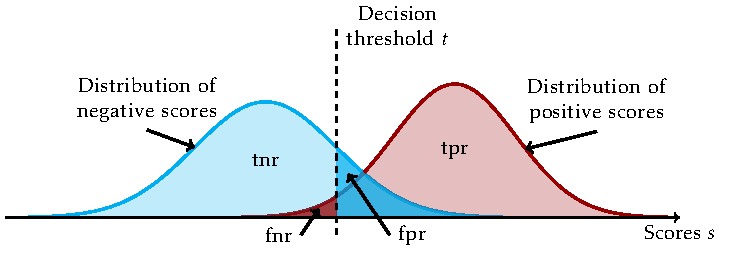
\includegraphics{../images/confusion_rates.pdf}
  \end{center}
\end{frame}

\begin{frame}{Classifier 1 is better ... or not?}
  \begin{center}
    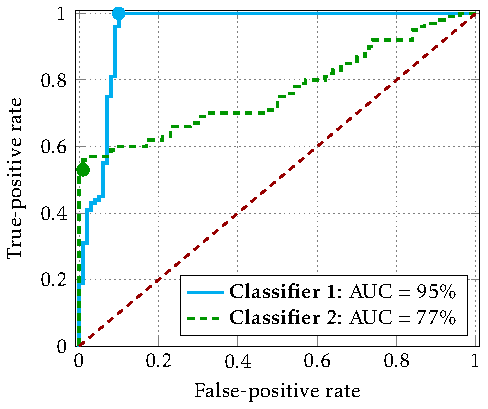
\includegraphics[width=\linewidth, height=0.9\textheight, keepaspectratio]{
      ../images/roc_space_presentation.pdf
    }
  \end{center}
\end{frame}


\begin{frame}{Sometimes Classifier 2 is the better one...}
  \begin{center}
    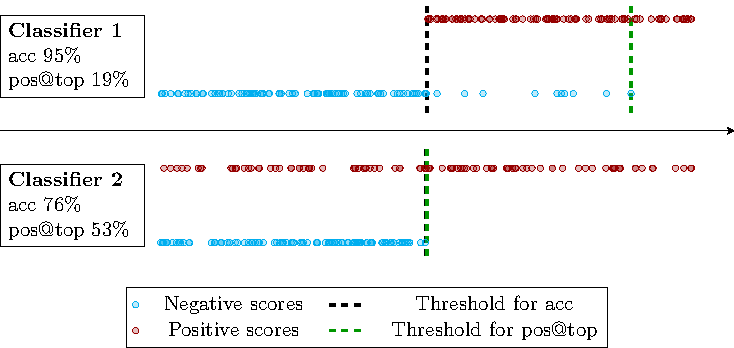
\includegraphics[width=\linewidth, height=0.9\textheight, keepaspectratio]{
      ../images/standard_aatp_comparison.pdf
    }
  \end{center}
\end{frame}

\section{Classification at the Top}

\begin{frame}{General problem formulation}
  \begin{itemize}
    \item \textbf{Goal:} correctly classify only the most relevant samples. The most relevant samples are samples with the highest scores
    \item General formulation
    \begin{mini*}{\bm{w}}{
      C_1 \sum_{i \in \Ineg} {\color{myorange}\Iverson{s_i \geq t}} + C_2 \sum_{i \in \Ipos} {\color{myorange}\Iverson{s_i < t}}
    }{}{}
      \addConstraint{s_i}{= {\color{mypurple}f(\bm{x}_i; \bm{w})}, \quad}{i \in \I}
      \addConstraint{t}{= {\color{mygreen}G\Brac{\bm{s}, \bm{y}}}}
    \end{mini*}
    where threshold~$t$ is a function of all scores
    \item Difficult problem: constrained, {\color{myorange}discontinuous}, generally {\color{mypurple}non-convex}, and {\color{mygreen}non-decomposable}
  \end{itemize}
\end{frame}

\begin{frame}{How to get continuous objective function?}
  \begin{itemize}
    \item By replacing~${\color{myorange}\Iverson{\cdot{}}}$ Iverson function with its surrogate approximation
  \end{itemize}
  \begin{center}
    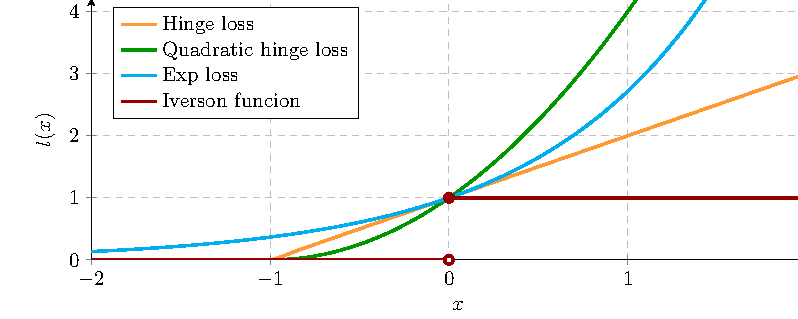
\includegraphics[width=\linewidth, height=0.7\textheight, keepaspectratio]{
      ../images/surrogates.pdf
    }
  \end{center}
\end{frame}


\begin{frame}{General surrogate formulation}
  \begin{itemize}
    \item Using the surrogate approximation to replace~${\color{myorange}\Iverson{\cdot{}}}$  leads to the general surrogate formulation
    \begin{mini*}{\bm{w}}{
      C_1 \sum_{i \in \Ineg} {\color{myorange}l(s_i - t)} + C_2 \sum_{i \in \Ipos} {\color{myorange}l(t - s_i)}
    }{}{}
      \addConstraint{s_i}{= f(\bm{x}_i; \bm{w}), \quad}{i \in \I}
      \addConstraint{t}{= G\Brac{\bm{s}, \bm{y}}}
    \end{mini*}
  \end{itemize}
\end{frame}

\begin{frame}{How to choose the decision threshold?}
  \begin{itemize}
    \item For simplicity, we focus only on formulations that minimize the false-negative rate and the threshold function~${\color{mygreen}G}$ depends only on negative samples
    \begin{mini*}{\bm{w}}{
      \frac{1}{2} \norm{\bm{w}}^2 + \frac{1}{\npos} \sum_{i \in \Ipos} l(t - s_i)
    }{}{}
      \addConstraint{s_i}{= f(\bm{x}_i; \bm{w}), \quad}{i \in \I}
      \addConstraint{t}{= {\color{mygreen}G\Brac{\bm{s}, \bm{y}}}}
    \end{mini*}
    where we use~$C_1 = 0$ and~$C_2 = \frac{1}{\npos}.$ Regularization is added for numerical stability.
    \item<2-> \TopPush maximizes the number of positive samples at the top 
    \begin{equation*}
      t = {\color{mygreen}G_{TopPush}\Brac{\bm{s}, \bm{y}}} = \max_{j \in \Ineg} s_j
    \end{equation*}
    \item<3-> \PatMatNP maximizes true-positive rate with fixed false-positive rate 
    \begin{equation*}
      t = {\color{mygreen}G_{Pat\&Mat-NP}\Brac{\bm{s}, \bm{y}}} \;\; \iff \;\;  t \;\; \text{solves} \;\; \frac{1}{\nneg}\sum_{i \in \Ineg} l\Brac{s_i - t} = \tau
    \end{equation*}
  \end{itemize}
\end{frame}

\section{Classification at the Top: \\ Linear Model}

\begin{frame}{Linear Model}
  \begin{itemize}
    \item General surrogate formulation with linear model~${\color{mypurple}f(\bm{x}; \bm{w}) = \bm{w}^{\top} \bm{x}}$
    \begin{mini*}{\bm{w}}{
      \frac{1}{2} \norm{\bm{w}}^2 + \frac{1}{\npos} \sum_{i \in \Ipos} l(t - s_i)
    }{}{}
      \addConstraint{s_i}{= {\color{mypurple}\bm{w}^{\top} \bm{x}_i}, \quad}{i \in \I}
      \addConstraint{t}{= G\Brac{\bm{s}, \bm{y}}}
    \end{mini*}
    \item Properties that we are interested in:
    \begin{itemize}
      \item Convexity of the objective function
      \item Robustness to outliers
    \end{itemize}
  \end{itemize}
\end{frame}

\begin{frame}{Convexity of the objective function}
  \begin{block}{Theorem}
    If the threshold $t$ is a convex function of the weights $\bm{w},$ then function
    \begin{equation*}
      L(\bm{w}) = \frac{1}{2} \norm{\bm{w}}^2 + \frac{1}{\npos} \sum_{i \in \Ipos} l(t(\bm{w}) - \bm{w}^{\top} \bm{x}_i)
    \end{equation*}
    is convex.
  \end{block}
  \begin{itemize}
    \item What does it mean? 
    \begin{itemize}
      \item Both formulations \TopPush and \PatMatNP have convex thresholds
      \item Both formulations are convex and continuous
      \item We can solve both formulations using gradient descent algorithm
    \end{itemize}
    
  \end{itemize}
\end{frame}

\begin{frame}{How to solve it?}
  \begin{itemize}
    \item Using gradient descent
    \begin{equation*}
      \bm{w}^{k+1} \gets \bm{w}^k - \alpha^k \cdot \nabla L(\bm{w}^k),
    \end{equation*}
    where~$\alpha^k > 0$ is a learning rate, and~$\nabla L(\bm{w}^k)$ is a gradient of the objective function
    \begin{equation*}
      \nabla L(\bm{w})
        = \bm{w} + \frac{1}{\npos} \sum_{i \in \Ipos} l'\Brac{{\color{mygreen}t(\bm{w})} - {\color{mypurple}\bm{w}^{\top} \bm{x}_i}}\Brac{{\color{mygreen}\nabla t(\bm{w})} - {\color{mypurple}\bm{x}_i}}
    \end{equation*}
    \item How to compute gradient of the threshold~${\color{mygreen}\nabla t(\bm{w})}$?
    \begin{itemize}
      \item For \TopPush it is easy
      \begin{equation*}
        j^{\star} = \arg \max_{j \in \Ineg} s_j \quad \rightarrow \quad 
        t = s_{j^{\star}}\quad \rightarrow \quad 
        {\color{mygreen}\nabla t(\bm{w})} = \nabla f(\bm{x}_{j^{\star}}; \bm{w}) = \bm{x}_{j^{\star}}
      \end{equation*}
      \item For \PatMatNP we have to use {\color{mygreen}\textbf{implicit function theorem}}.
    \end{itemize}
  \end{itemize}
\end{frame}

\begin{frame}{When convexity is not enough...}
  \begin{center}
    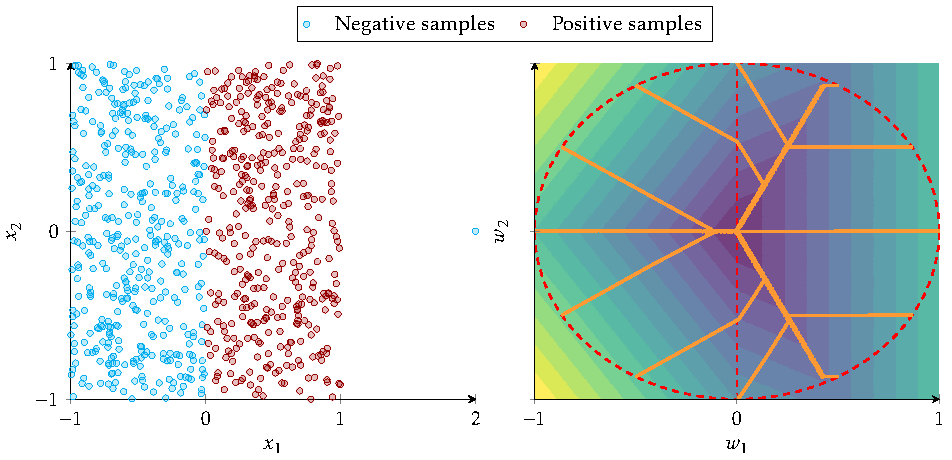
\includegraphics[width=\linewidth, height=0.9\textheight, keepaspectratio]{
      ../images/toppush_convergence.pdf
    }    
  \end{center}
\end{frame}

\section{Classification at the Top: \\ Non-linear Model}

\begin{frame}{Non-linear Model}
  \begin{itemize}
    \item General surrogate formulation with non-linear model~${\color{mypurple}f(\bm{x}; \bm{w})}$
    \begin{mini*}{\bm{w}}{
      \frac{1}{2} \norm{\bm{w}}^2 + \frac{1}{\npos} \sum_{i \in \Ipos} l(t - s_i)
    }{}{}
      \addConstraint{s_i}{= {\color{mypurple}f(\bm{x}_i; \bm{w})}, \quad}{i \in \I}
      \addConstraint{t}{= G\Brac{\bm{s}, \bm{y}}}
    \end{mini*}
    \item Disadvantages:
    \begin{itemize}
      \item Objective function is not convex
      \item Non-linear models are usually large and expensive to train
    \end{itemize}
    \item What to do if the dataset is too large to fit in memory? Stochastic gradient descent.
  \end{itemize}
\end{frame}

\begin{frame}{Issues with stochastic gradient descent}
  \begin{itemize}
    \item The threshold is a function of all scores $\rightarrow$ the loss function is non-decomposable
    \item As a result, stochastic gradient descent provides a biased gradient estimate
  \end{itemize}
  \begin{center}
    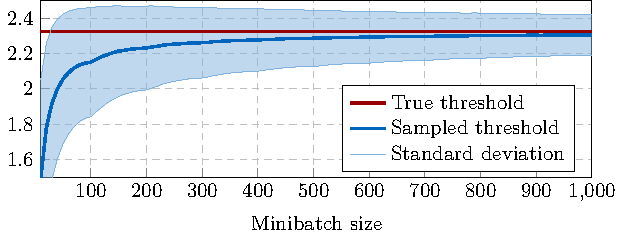
\includegraphics[width=\linewidth, height=0.6\textheight, keepaspectratio]{
      ../images/deep_threshold_bias.pdf
    }
  \end{center}
  \begin{itemize}
    \item How to reduce bias? Increase size of minibatch ...
  \end{itemize}
\end{frame}

\begin{frame}{Is there a better way to reduce bias?}
  \begin{itemize}
    \item \DeepTopPush: Add threshold from last minibatch
    \begin{equation*}
      j^{\star} = \arg \max_{j \in \Ineg} s_j \quad \rightarrow \quad 
      t = s_{j^{\star}}\quad \rightarrow \quad 
      \nabla t(\bm{w}) = {\color{mypurple}\nabla f(\bm{x}_{j^{\star}}; \bm{w})}
    \end{equation*}
  \end{itemize}
  \begin{center}
    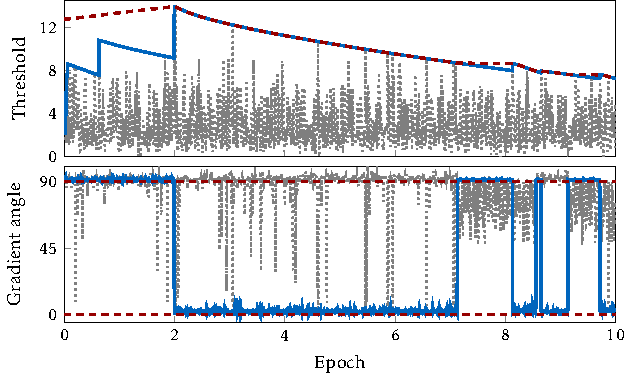
\includegraphics[width=\linewidth, height=0.75\textheight, keepaspectratio]{
      ../images/deep_thresholds.pdf
    }
  \end{center}
\end{frame}

\section{How does it work?}

% \begin{frame}{Steganalysis}
%   \begin{itemize}
%     \item Train data: 186 583 samples, 9.1\% of samples are positive
%     \item Test data: 248 776 samples, 9.1\% of samples are positive
%     \item Each sample consists of 22 510 features
%     \item Only linear model
%     \item \textbf{Goal:}
%     \begin{itemize}
%       \item Maximize the true-positive rate at very low levels of the false-positive rate
%     \end{itemize}
%   \end{itemize}
% \end{frame}

\begin{frame}{Steganalysis}
  \begin{center}
    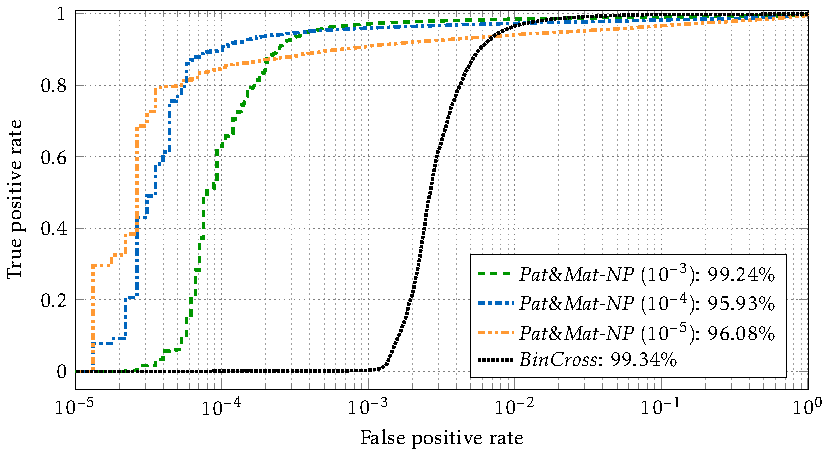
\includegraphics[width=\linewidth, height=0.9\textheight, keepaspectratio]{
      ../images/stego_nsft5.pdf
    }
  \end{center}
\end{frame}

% \begin{frame}{AVAST: Malware detection}
%   \begin{itemize}
%     \item Train data: 6 580 166 samples, 87.2\% of samples are positive
%     \item Test data: 800 346 samples, 91.8\% of samples are positive
%     \item Hierarchical data structure:
%     \begin{itemize}
%       \item Each sample is a JSON file, which may consist of other JSON files
%       \item Each sample is of a different size (from 1 KB to 2.5 MB)
%       \item \DeepTopPush and \PatMatNP used as an extension for hierarchical multi-instance learning (HMIL)
%     \end{itemize}
%     \item \textbf{Goal:}
%     \begin{itemize}
%       \item Maximize the true-positive rate at extremely low levels of the false-positive rate to avoid disruptive false alarms for the end-user.
%     \end{itemize}
%   \end{itemize}
% \end{frame}

\begin{frame}{AVAST: Malware detection}
  \begin{center}
    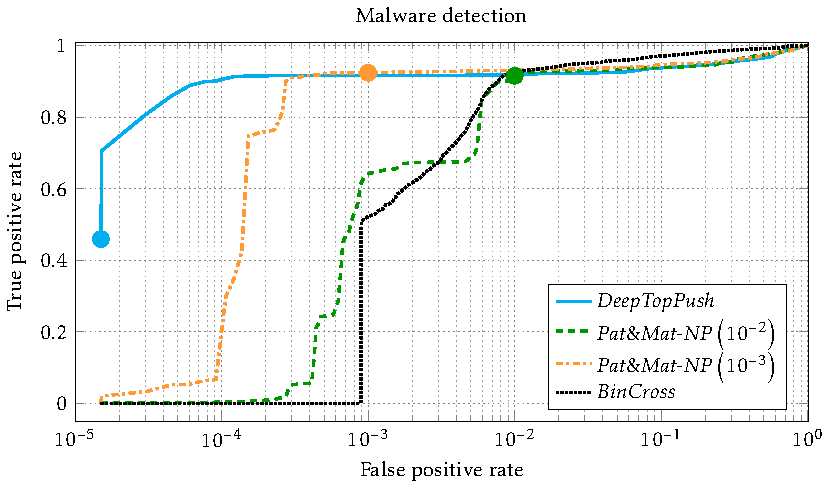
\includegraphics[width=\linewidth, height=0.9\textheight, keepaspectratio]{
      ../images/malware_detection.pdf
    }
  \end{center}
\end{frame}

\section{Main contributions}

\begin{frame}{Contributions}
  \begin{itemize}
    \item \textbf{Unification Contributions:}
    \begin{itemize}
      \item Introduction of a unified framework for Classification at the Top
      \item Showed that problems such as Ranking or Accuracy at the Top fall into the framework
      \item Introduction of \PatMat and \PatMatNP formulations
    \end{itemize}
    \item \textbf{Theoretical Contributions:}
    \begin{itemize}      
      \item Derivation of theoretical properties of formulations from the framework with linear model
      \item Derivation of dual forms and use of non-linear kernels
    \end{itemize}
    \item \textbf{Algorithmic Contributions:}
    \begin{itemize}
      \item Derivation of an efficient algorithm for solving dual forms
      \item Introduction of a modified stochastic gradient descent
      \item Introduction of \DeepTopPush formulation
    \end{itemize}
  \end{itemize}
\end{frame}

\section{Thank you for your attention.}

\end{document}
